\documentclass[11pt]{article}
\usepackage{graphicx}
\usepackage{amsmath}
\usepackage{listings}
\graphicspath{ {./} }
\setcounter{secnumdepth}{0}

\begin{document}
\begin{titlepage}
   \begin{center}
       \vspace*{1cm}
       \textbf{\Huge Numerical Methods} \\
       \vspace{2.0cm}
       \huge{ProjectAssignment A: Accuracy of computation} \\
       \vspace{.7cm}
       \huge{\today} \\
       \vspace{3.0cm}
       \vspace{0.4cm}
       Krzysztof Watras\\
       \vspace{ 0.2cm }
       \small{ Tutor's name: Jakub Wagner } \\
       \vspace{2 cm}   
       \small{Computer Science} \\  
       \vspace{0.2cm}       
       \small{Warsaw University of Technology,\\
       Faculty of Electronics and Technology} \\
       \vspace{2cm}
       \small{I declare that this piece of work, which is the basis for
       recognition of achieving learning outcomes in the Numerical Methods
       course, was completed on my own. Krzysztof Watras} \\
   \end{center}
\end{titlepage} 
\tableofcontents

\newpage
\section{Introduction}
In this report I submit results of first assignment from ENUME course. This 
assignment focuses on the errors introduced during the numerical calculation
due to inaccurate floating point representation standards. All tasks that are
to be performed involve the same equation:
$$y = \frac{\cos(x)}{x^3} - x^2$$

Task 1 is focused on calculating the error introduced by the inaccurate storage
of floating point numbers itself. This error will be noted as $\epsilon$. This
error will be different for different values of $x$, and so we will call it
$T(x)$, to make clear that this property depends on $x$. Task 2 and task 3
focus on the error introduced by inaccurate representation of intermediate
results. This error will be noted as $\eta$.  Additionally, the tasks try to
analyze, how different methods result in total error introduced to the final
result. Here we will use $K_{a1}(x)$ and $K_{a2}(x)$ to differentiate it from
error obtained in task 1 and from each other.

Throughout the document I will use following convention for two methods of
calculating the results:
\begin{itemize}
    \item \textbf{Analytical} when I am using the epsilon calculus to obtain results \\
    \item \textbf{Numerical} when I am using the method of simulation implemented as instructed in the assignment \\
\end{itemize}
This schema may be seen as slightly inaccurate, but it is consistent throughout 
the document, and it therefore considered best to avoid confusion and repetition

\section{Mathematical Symbols and formulas used}
\begin{equation}
    \sigma [\tilde{v}^k] = T^k \cdot \sigma[\tilde{v}^{k-1}] + \eta^k
    \label{eq:generaleq}
\end{equation}
\begin{equation}
    For\ \alpha \to 0,\sin(\alpha)\approx\alpha -\frac{\alpha^3}{6},\cos(\alpha)\approx 1-\frac{\alpha^2}{2}
    \label{eq:trigapprox}
\end{equation}
\begin{equation}
    \begin{align}
        (1+\epsilon_1)(1+\epsilon_2) &\approx 1 + \epsilon_1 + \epsilon_2 \\
        (1+\epsilon_1)^a &\approx 1 + a\epsilon_1 \\
    \end{align}
    \label{eq:epsilonapprox}
\end{equation}
\begin{equation}
    \begin{align}
        For\ \sigma[\tilde{y}] &\approx 
        T_1\epsilon_1 +  T_2\epsilon_2 +  T_3\epsilon_3 + \dots  \\
        & + K_1\eta_1 +  K_2\eta_2 +  K_3\eta_3 + \dots \\
        T_x &= \left|T_1\right| + \left|T_2\right| + \left|T_3\right| + \dots \\
        K_x &= \left|K_1\right| + \left|K_2\right| + \left|K_3\right| + \dots \\
    \end{align}
    \label{eq:approxerrors}
\end{equation}

Properties (\ref{eq:generaleq},\ref{eq:epsilonapprox},\ref{eq:approxerrors})
is introduced to us in the ENUME Lecture Notes[1].

Property (\ref{eq:trigapprox}) stems from the Tailor series of those functions[2].

\section{Description of the numerical methods and algorithms}
\subsection{Inline Functions}
In my calculations I use inline functions as they allow me to more easily
express the intent. This is because I do not have to create separate files and
perform linking of some sort in order to do computation. For general syntax of
Inline functions you may refer to official MATLAB documentation[3].

Inline functions I use:
\begin{lstlisting}[language=MATLAB]
    y = @(x) cos(x)./x.^3 - x.^2;
\end{lstlisting}
is just a MATLAB representation of the function we analyze in the report.
\begin{lstlisting}[language=MATLAB]
    rand_sign_vec = @() (randi(2,1,5)-1.5)*2;
\end{lstlisting}
Is a custom function that returns a matrix of size 1x5 (so a vector length 5)
of random numbers, either -1 or 1. Spread of both should be uniform as this uses
builtin function `randi` that according to documentation[4] does exactly what one
would expect it to. To clarify what is happening: first we choose number: 1 or 2,
then we shift it to -0.5 or 0.5, then we scale it to -1 or 1.

\subsection{Method of calculating the maximal error from random trials}
\begin{lstlisting}[language=MATLAB]
    tx_numerical = zeros(1, 100);
    rand_sign_vec = @() (randi(2,1,5)-1.5)*2;
    for i = 1:300
        en = eta * rand_sign_vec();
        v1 = T1 * (1+en(1));
        v2 = T1 * (1+en(2));
        v3 = T1 * (1+en(3));
        v4 = T2 * (1+en(4));
        v5 = (1+en(5));
        ytilde = v1+v2+v3+v4+v5;
        tx_numerical = max(tx_numerical, ytilde);
    end
\end{lstlisting}
This is the code that is responsible for calculations in tasks 2 (very similar in task 3). 
First, we initialize the array of 100 zeros, then we enter a loop and repeat 300 times:
\begin{enumerate}
    \item Create an array of random numbers
    \item Multiply the vector by eta
    \item Multiply each component of the answer by the $\pm$ eta
    \item Sum all components
    \item Update max error table
\end{enumerate}

\newpage
\section{Task 1}
Given a function $$y = \frac{\cos(x)}{x^3} - x^2$$ we want to calculate total
error introduced by inaccurate representation of $x$.
\subsection{Epsilon calculus}
To calculate error of representation, everywhere where there is an $x$, we need
to introduce $\epsilon$ as the error like so: $\tilde{x} = x(1+\epsilon)$
In our function we have:
\begin{align*}
    v_1 &= \cos(x) \\ 
    v_2 &= x^3 \\ 
    v_3 &= \frac{v_1}{v_2} \\ 
    v_4 &= x^2 \\ 
    y &= v_3 - v_4
\end{align*}
Therefore we obtain:
\begin{align*}
    \tilde{v_1} &= \cos(x(1+\epsilon_1)) \\ 
    \tilde{v_2} &= (x(1+\epsilon))^3 = x^3 (1+3\epsilon_2) \\ 
    \tilde{v_3} &= \frac{\tilde{v_1}}{\tilde{v_2}} \\ 
    \tilde{v_4} &= (x(1+\epsilon))^2 = x^2 (1+2\epsilon_3) \\
    \tilde{y} &= \tilde{v_3} - \tilde{v_4}
\end{align*}
Let us focus on $\tilde{ v_1 }$:
$$ \cos(x(1+\epsilon)) = \cos(x+x\epsilon) = \cos(x)\cos(x\epsilon) -
\sin(x)\sin(x\epsilon) $$
We need to use properties of trigonometric functions in order to solve it.
Those properties are listed in the section \textit{Mathematical Symbols and
formulas used}, formula (2). \\
Using those properties:
\begin{align*}
    \cos(x(1+\epsilon)) &= \cos(x)\cos(x\epsilon) - \sin(x)\sin(x\epsilon)\\
    &= \cos(x)(1-\frac{(x\epsilon)^2}{2}) - \sin(x)(x-\frac{(x\epsilon)^3}{6})\epsilon \\
    &= \cos(x) - \sin(x)x\epsilon\\
    &= \cos(x)\cdot (1-\tan(x)x\epsilon)
\end{align*}
Now solve $v_3$:
\begin{align*}
    \tilde{v_3} &= \displaystyle\frac{\cos(x) \cdot (1 - x\tan(x)
    \epsilon_1)}{x^3 (1+3\epsilon_2)}\\
    &= \frac{\cos(x)}{x^3} (1 - x\tan(x) \epsilon_1)\cdot (1+3\epsilon_2)^{-1}\\
    &= \frac{\cos(x)}{x^3} (1 - x\tan(x) \epsilon_1)\cdot (1-3\epsilon_2)\\
    &= \frac{\cos(x)}{x^3} (1 - x\tan(x) \epsilon_1 - 3\epsilon_2)
\end{align*}
Substituting it to the equation:
\begin{align*}
\tilde{y}&=\frac{\cos(x)}{x^3}(1 - x\tan(x) \epsilon_1 - 3\epsilon_2)-x^2(1+2\epsilon_3)\\
    &=\frac{\cos(x)}{x^3}-\frac{\cos(x)}{x^3}(x\tan(x) \epsilon_1 +
    3\epsilon_2)-x^2-2x^2\epsilon_3 \\
    &=y-\frac{\cos(x)}{x^3}(x\tan(x) \epsilon_1 + 3\epsilon_2)-2x^2\epsilon_3\\
    &=y(1 + (-\frac{\cos(x)}{x^3}(x\tan(x) \epsilon_1 +
    3\epsilon_2)-2x^2\epsilon_3)\frac1y)\\
    &=y\left(1 + \left(-\frac{\sin(x)}{x^2}\epsilon_1
    -3\frac{\cos(x)}{x^3}\epsilon_2 - 2x^2\epsilon_3\right)\frac1y\right)
\end{align*}
Therefore, using the formula (4):
$$T(x) = \displaystyle\frac{ \left|-\frac{\sin(x)}{x^2}\right| +
\left|- 3\frac{\cos(x)}{x^3}\right| + \left|-2x^2\right| }
{\frac{\cos(x)}{x^3} - x^2}$$

\subsection{Numerical simulation}
Function that we need to implement, described in an assignment:
$$T(x) = \frac{1}{\epsilon_{sim}}\left| \displaystyle\frac{y(\tilde{x}) - y(x)}{y(x)} \right|$$
is more general solution for calculating the error. It can be easily implemented 
in MATLAB code:
\begin{lstlisting}[language=MATLAB]
    y = @(x) cos(x)./x.^3 - x.^2;
    x_eps = x.*(1+esim);
    yeps = y(x_eps);
\end{lstlisting}
where anonymous function y can be reused for calculating "true" value of the function.

\subsection{Comparison of results}
Both methods do not differ significantly from one another in terms of results.
This can be seen on \ref{fig:task1}, where the output difference is barely
noticable. Therefore, the use of simpler solution should be recommended.
\begin{figure}[ht]
    \begin{center}
        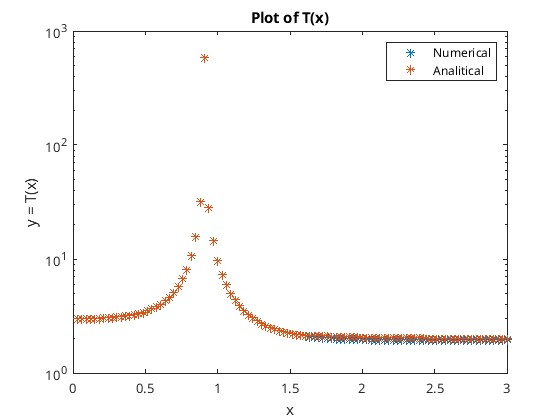
\includegraphics[width=\textwidth]{Task1.jpg}
    \end{center}
    \caption{Comparison of calculating error via numerical and analytical way}
    \label{fig:task1}
\end{figure}


\newpage
\section{Task 2}
Conveniently, in task 2 we have the same function and same name for each $v_n$ 
component as we did in Task 1. Therefore, we just need to change the part where 
we introduce errors:
\begin{align*}
    \tilde{v_1} &= \cos(x) (1+\eta_1)\\ 
    \tilde{v_2} &= x^3(1+\eta_2)\\ 
    \tilde{v_3} &= \frac{\tilde{v_1}}{\tilde{v_2}}(1+\eta_3) \\ 
    \tilde{v_4} &= x^2 (1+\eta_4) \\
    \tilde{y} &= (\tilde{v_3} - \tilde{v_4})(1+\eta_5)
\end{align*}
\subsection{Epsilon calculus}
Using the epsilon calculus rules:
\begin{align*}
    \tilde{y} &= \left(
    \frac{\cos(x)}{x^3}\frac{(1+\eta_1)}{(1+\eta_2)}(1+\eta_3) - x^2(1+\eta_4)
    \right) (1+\eta_5) \\
    &= \left(\frac{\cos(x)}{x^3}(1+\eta_1-\eta_2+\eta_3) - x^2(1+\eta_4)\right)(1+\eta_5)\\
    &= y \left(1+ \frac{\cos(x)}{x^3}\frac1y(\eta_1-\eta_2+\eta_3) - x^2\frac1y\eta_4 \right)(1+\eta_5) \\
    &= y \left(1+ \frac{\cos(x)}{x^3}\frac1y(\eta_1-\eta_2+\eta_3) - x^2\frac1y\eta_4 + \eta_5\right) \\
\end{align*}
Finally, we get:
\begin{align*}
K_{A1} &= \displaystyle\frac{
    \left|\frac{\cos(x)}{x^3}\right| + 
    \left|-\frac{\cos(x)}{x^3}\right| +
    \left|\frac{\cos(x)}{x^3}\right| + 
    \left|-x^2\right|}
{\left|\frac{\cos(x)}{x^3} - x^2\right|} + 1\\
\end{align*}

\subsection{Numerical simulation}
In this exercise we simulate the error that we get due to rounding errors.
Here, it is important to note that some errors may interfere such that they add
up, or cancel out. Ideally we would try to calculate each permutation of
$-\eta$ and $+\eta$, as that would yield true max error. However, in practice,
it may take too long to calculate full coverage. Often, we may want to know
just "good enough" approximation of this error. Therefore, we try a number of
randomly selected sample and calculate the error by updating the biggest error.
Exact code solution can be seen in \textit{Description of the numerical methods
and algorithms} section.

\subsection{Comparison of results}
Similarly to results of task 1, both methods do not differ significantly from
one another in terms of results. This can be seen on \ref{fig:task2}, where the
output difference cannot even be seen (due to one point drawn on the other).

\begin{figure}[ht]
    \begin{center}
        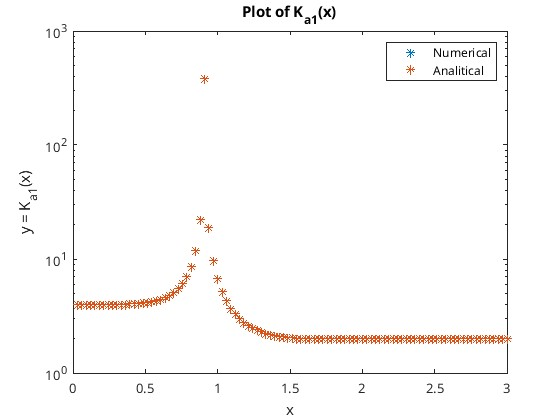
\includegraphics[width=\textwidth]{Task2.jpg}
    \end{center}
    \caption{Comparison of calculating error via numerical and analytical way}
    \label{fig:task2}
\end{figure}


\newpage
\section{Task 3}
\begin{align*}
    v_1 &= \cos(x) \\ 
    v_2 &= x^5 \\ 
    v_3 &= v_1-v_2 \\ 
    v_4 &= x^3 \\ 
    y &= \frac{v_3}{v_4}
\end{align*}
Therefore:
\begin{align*}
    \tilde{v_1} &= \cos(x) (1+\eta_1)\\ 
    \tilde{v_2} &= x^5(1+\eta_2)\\ 
    \tilde{v_3} &= (\tilde{v_3} - \tilde{v_4})(1+\eta_3) \\ 
    \tilde{v_4} &= x^3 (1+\eta_4) \\
    \tilde{y} &= \frac{\tilde{v_3}}{\tilde{v_4}}(1+\eta_5)
\end{align*}
\subsection{Epsilon calculus}
Using the epsilon calculus rules:
\begin{align*}
    \tilde{y} &= \left(
    \displaystyle\frac{\cos(x)(1+\eta_1) - x^5(1+\eta_2)(1+\eta_3)}
    {x^3(1+\eta_4)}
    \right) (1+\eta_5) \\
    &=\displaystyle\frac{\cos(x)(1+\eta_1+\eta_3-\eta_4+\eta_5)-
    x^5(1+\eta_2+\eta_3-\eta_4+\eta_5)}{x^3}\\
    &=\displaystyle\frac{\cos(x)+cos(x)(\eta_1+\eta_3-\eta_4+\eta_5)-
    x^5-x^5(\eta_2+\eta_3-\eta_4+\eta_5)}{x^3}\\
    &=y+\displaystyle\frac{cos(x)\eta_1+cos(x)(\eta_3-\eta_4+\eta_5)-
    x^5\eta_2-x^5(\eta_3-\eta_4+\eta_5)}{x^3}\\
    &=y+\displaystyle\frac{cos(x)\eta_1-x^5\eta_2+
    (cos(x)-x^5)(\eta_3-\eta_4+\eta_5)}{x^3}\\
    &=y\cdot\left(1+\frac{cos(x)}{x^3}\frac1y\eta_1-x^2\frac1y\eta_2+
    \frac{cos(x)-x^5}{x^3}\frac1y(\eta_3-\eta_4+\eta_5)\right)\\
\end{align*}
Finally, we get:
$$ K_{A2} = \displaystyle\frac{
    \left|\frac{\cos(x)}{x^3}\right| + \left|-x^2\right|
+ \left| \frac{\cos(x)-x^5}{x^3} \right|
+ \left|-\frac{\cos(x)-x^5}{x^3} \right|
+ \left| \frac{\cos(x)-x^5}{x^3} \right|
} {\left|\frac{\cos(x)}{x^3} - x^2\right|}
$$

\subsection{Numerical simulation}
This part is identical to the corresponding one in Task 2. Of course the
components of the equation change but overall there is nothing to explain
further.

\subsection{Comparison of results}
Similarly to results of task 2, both methods do not differ significantly from
one another in terms of results. This can be seen on \ref{fig:task3}, where the
output difference cannot even be seen (due to one point drawn on the other).

\begin{figure}[ht]
    \begin{center}
        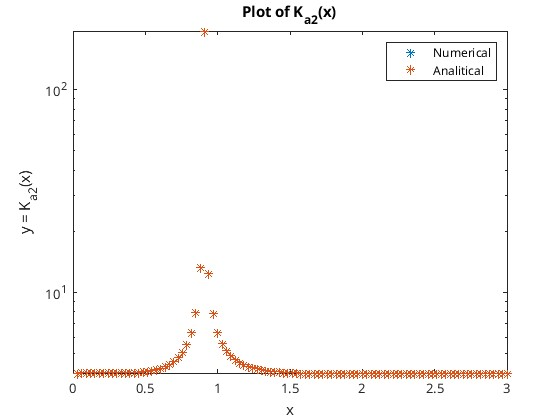
\includegraphics[width=\textwidth]{Task3.jpg}
    \end{center}
    \caption{Comparison of calculating error via numerical and analytical way}
    \label{fig:task3}
\end{figure}


\newpage
\section{Task 4 - Summary and Conclusions}

It's important to know that each floating point calculation if corrupted by
error so before analyzing the results it may be necessary to analyze if the
result is within satisfiable range of our precision. There is more to error of
the computation than just simple inaccuracy of value stored. Instead, each
calculation introduces more error.

\begin{figure}[ht]
    \begin{center}
        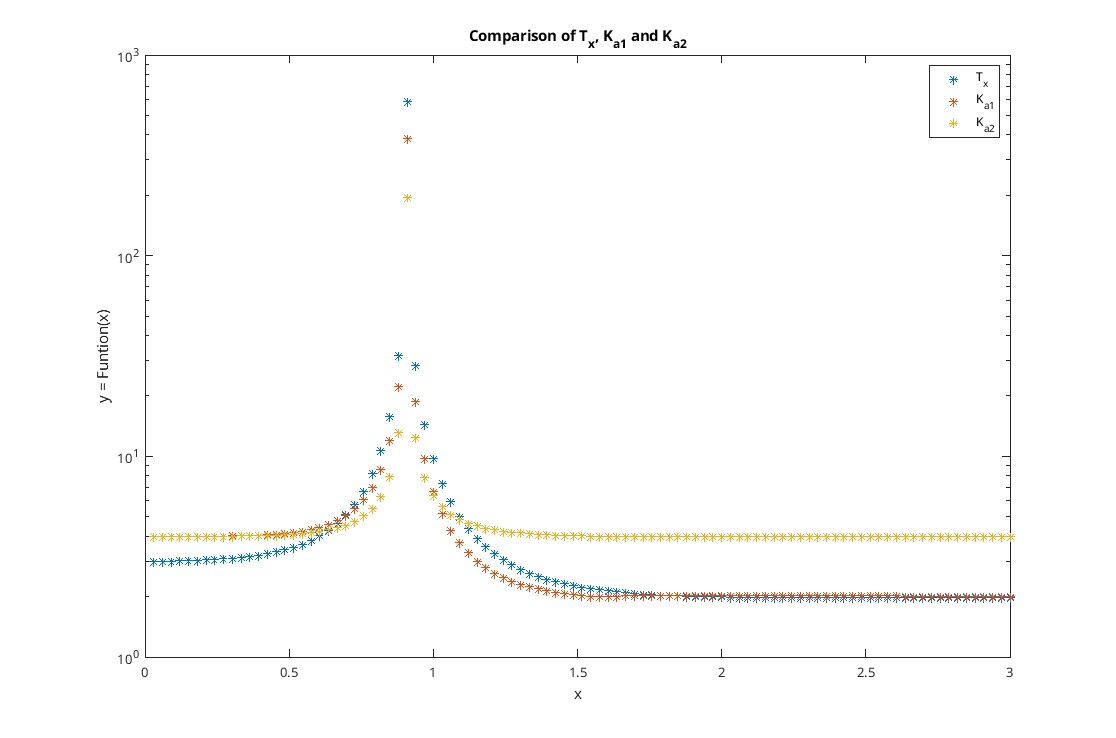
\includegraphics[width=\textwidth]{Task4.jpg}
    \end{center}
    \caption{Comparison of error from all 3 methods applied}
    \label{fig:task4}
\end{figure}

Different ways of calculating the same function can often have big impact on
the quality of the results. As one can clearly see from Figure \ref{fig:task4}
different methods yield different error results for the same input. In
particular, the difference between the $K_{a1}$ and $K_{a2}$, for $x\geq 1$ is
worthy of your attention. Furthermore, error introduced by the inaccurate
representation is different from the one that is introduced by the inaccurate
intermediate representation. Knowing that allows to design better, more
accurate algorithms. While developing and testing those methods it is ok to use
simplified formulas for calculating the error as they provide the same results
as the ones tailored to the specific problem.


\newpage
\section{References}
{[1]} R. Z. Morawski: Numerical methods (ENUME) – \emph{2. Accuracy and complexity of computing}, Warsaw University of Technology, Faculty of Electronics and Information Technology \\
{[2]} Tailor Series Table and definitions: \\https://people.math.sc.edu/girardi/m142/handouts/10sTaylorPolySeries.pdf
{[3]} Mathworks, official anonymous-function documentation: \\ https://www.mathworks.com/help/matlab/matlab_prog/anonymous-functions.html \\
{[4]} Mathworks, official anonymous-function documentation: \\ https://www.mathworks.com/help/releases/R2022b/matlab/ref/randi.html?searchHighlight=randi&s_tid=doc_srchtitle \\

\newpage
\section{Appendix: Listing of the developed programs}
\subsection{Source code for Task 1}
\lstinputlisting[language=MATLAB]{sol1.m}
\newpage
\subsection{Source code for Task 2}
\lstinputlisting[language=MATLAB]{sol2.m}
\newpage
\subsection{Source code for Task 3}
\lstinputlisting[language=MATLAB]{sol3.m}
\newpage
\subsection{Source code for Task 4}
\lstinputlisting[language=MATLAB]{sol4.m}

\end{document}

